\documentclass{beamer}
\usepackage{graphicx} % Required for inserting images
\usetheme{Madrid}

\title{Fabric Anomaly Detection}
\author{Jacopo Dardini \\ 
Gio Formichella}
\date{}

\usepackage{biblatex}
\addbibresource{refs.bib}

\setbeamertemplate{navigation symbols}{}  % Removes navitation symbols

\begin{document}

\frame{\titlepage}

\begin{frame}{Prato}
    \begin{columns}
        \begin{column}{0.5\textwidth}
            \begin{itemize}
                \item Fabric anomaly detection
                \item \textbf{Goal}: automate detection of mistakes in the production of cloth and textile material.
            \end{itemize}
            \begin{figure}
                \centering
                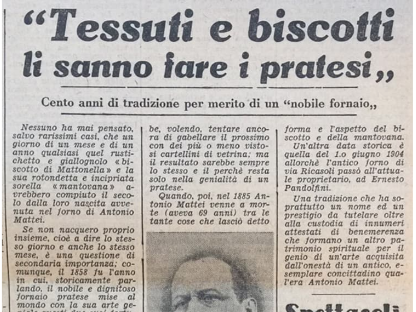
\includegraphics[width=1\linewidth]{imgs/giornale.png}
            \end{figure}
        \end{column}
        \begin{column}{0.5\textwidth}
            \begin{figure}
                \centering
                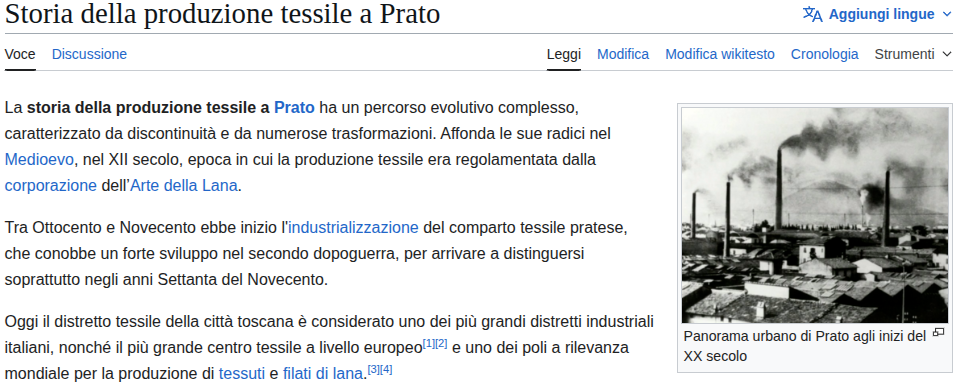
\includegraphics[width=1\linewidth]{imgs/storia_tessile_prato.png}
            \end{figure}
            \begin{figure}
                \centering
                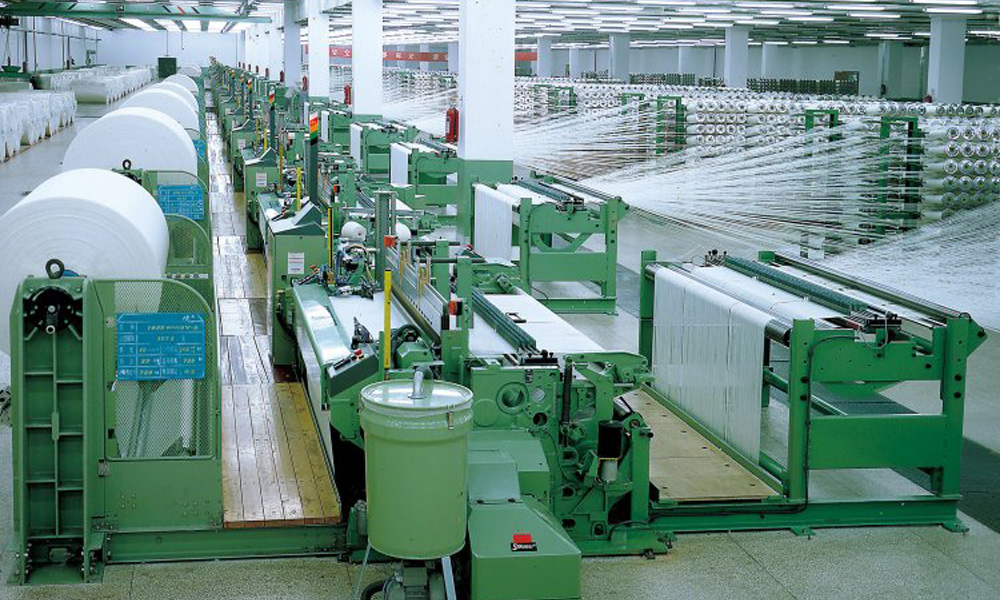
\includegraphics[width=1\linewidth]{imgs/macchinari.jpg}
            \end{figure}
        \end{column}
    \end{columns}
\end{frame}

\begin{frame}{Supervised vs Unsupervised Learning}
    \begin{itemize}
        \item The challenge with supervised learning in the textile industry is the \textbf{scarcity} of labeled anomalous data:
        \begin{itemize}
            \item Actively producing anomalous fabric is counterintuitive.
            \item Fabric design changes seasonally; at each shift, new anomalous data needs to be produced.
        \end{itemize}

        \vspace{0.3cm}
        \item Instead, unsupervised techniques like autoencoders exploit the large quantity of flawless fabric images and detect anomalies through the reconstruction error. We tested:
        \begin{itemize}
            \item \textbf{Convolutional autoencoders (CAE)}
            \item \textbf{Variational autoencoders (VAE)}
        \end{itemize}
    \end{itemize}
\end{frame}

\begin{frame}{Data}
\only<1>{
    \begin{itemize}
        \item We choose the fabric section of the \textbf{MVTec AD 2}\cite{MVTecAD2}.
        \item Dataset characteristics:
            \begin{itemize}
                \item Multiple different lighting conditions. Developed models will be robust to real-world distributions shifts due to illumination changes.
                \item High variability textures.
                \item Anomalies distributed across the entire height and width of the images and also directly appear on the image borders.
            \end{itemize}
        \item Defects:
        \begin{itemize}
            \item Cuts and holes.
            \item Color inconsistencies.
            \item Loose thread and extra fabric pieces.
        \end{itemize}
        \item \textbf{Main challenges}:
        \begin{itemize}
            \item Tiny defects with low contrast.
            \item High variability of the normal data due to varying pattern of the print.
        \end{itemize}
    \end{itemize}
}
\only<2-3>{
    \begin{itemize}
        \item Can you spot the anomalies ?
    \end{itemize}
    \begin{columns}<2-3>
        \begin{column}{0.5\textwidth}
            \begin{figure}
                \centering
                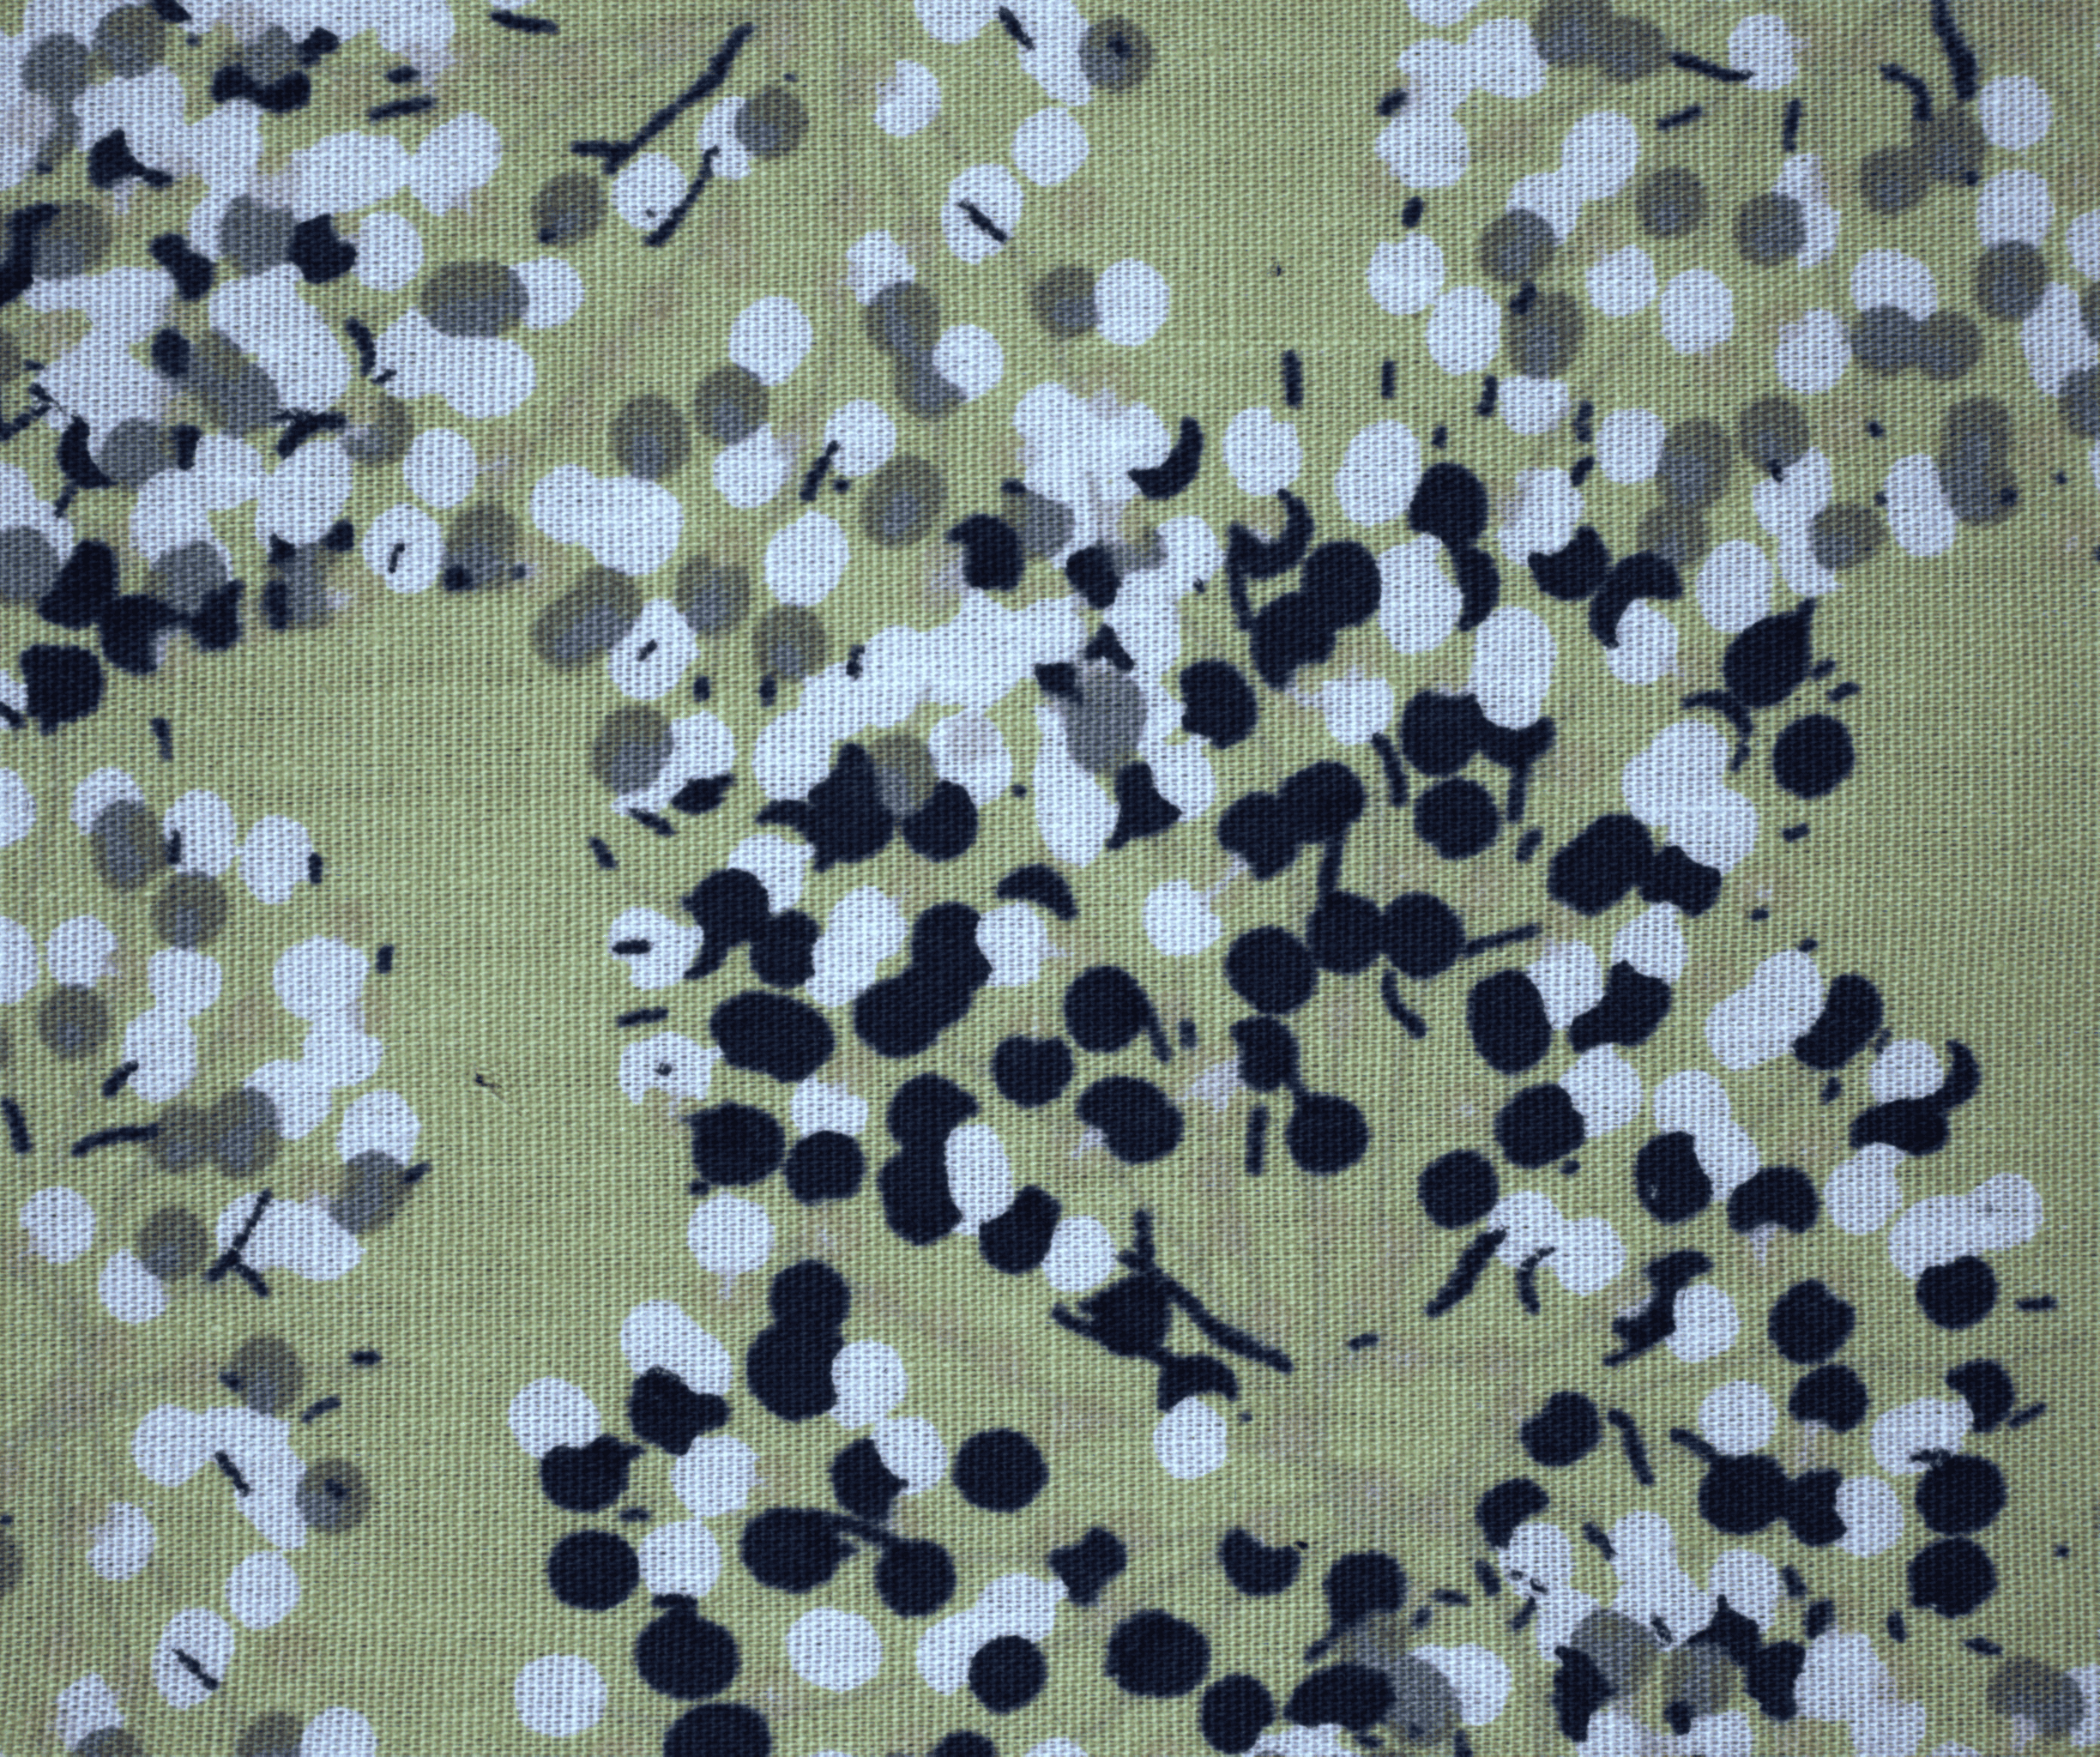
\includegraphics[width=1\linewidth]{imgs/005_overexposed.png}
            \end{figure}
        \end{column}
        \begin{column}{0.5\textwidth}<3>
            \begin{figure}
                \centering
                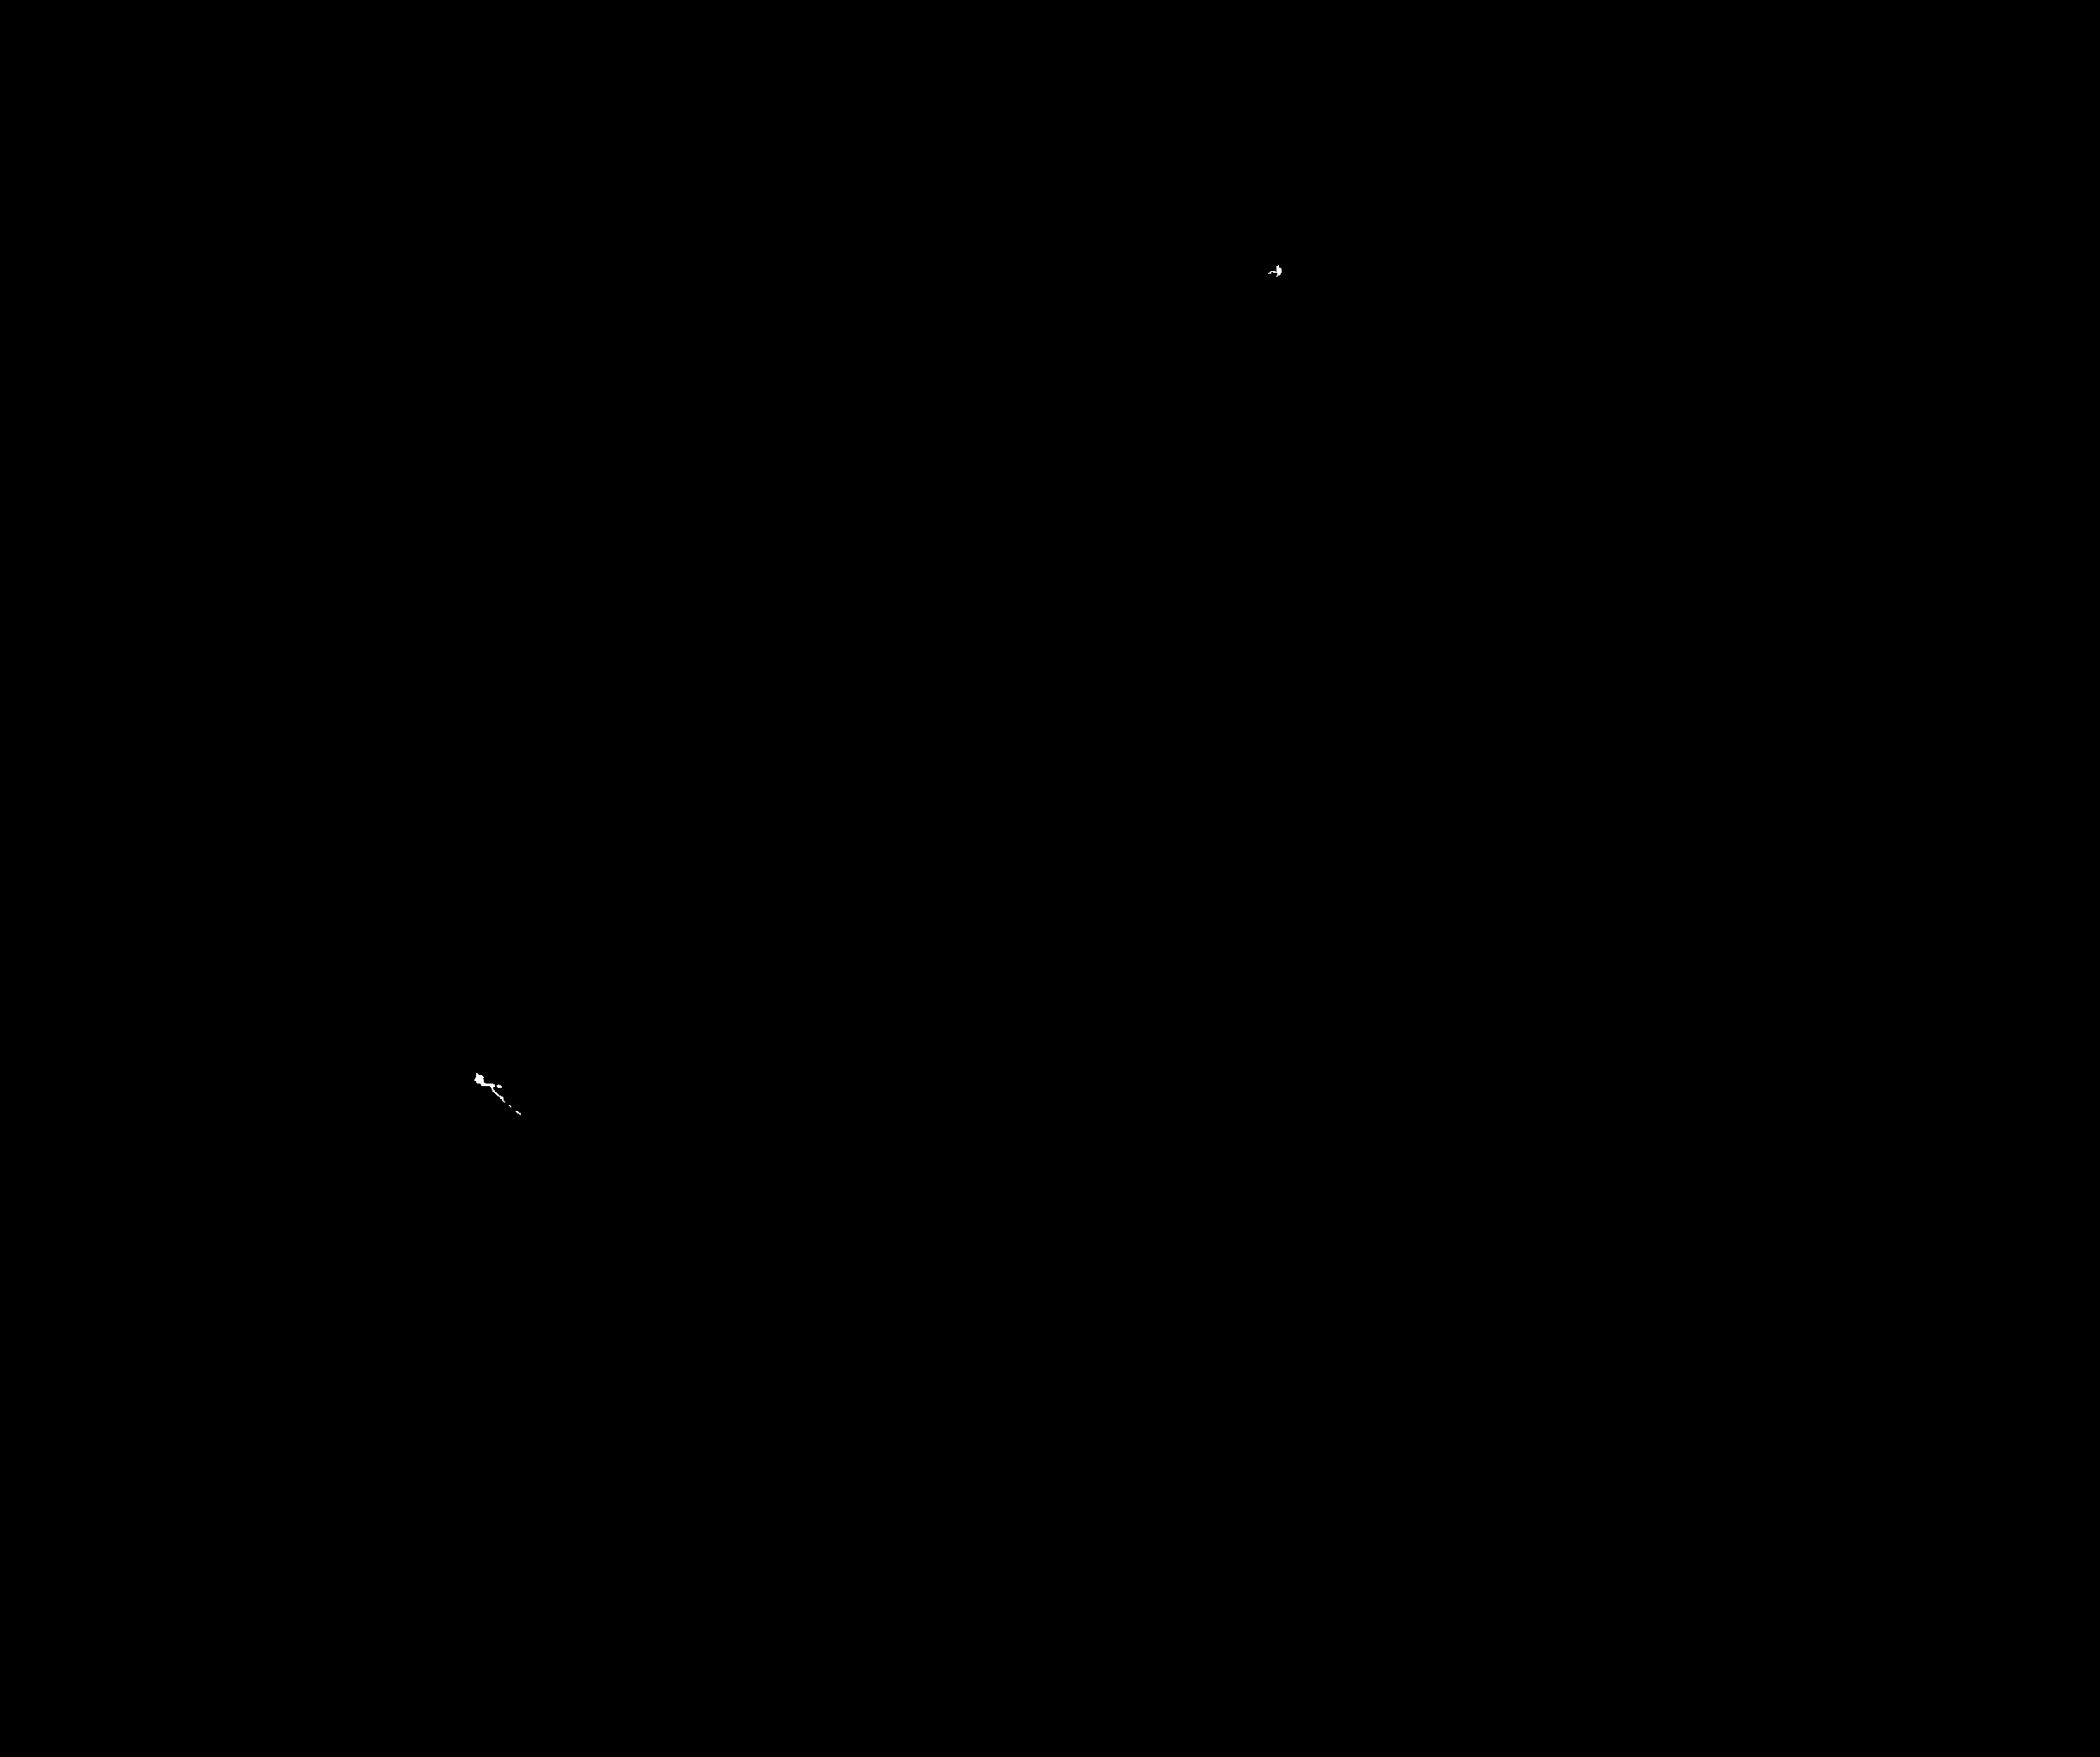
\includegraphics[width=1\linewidth]{imgs/005_overexposed_mask.png}
            \end{figure}
        \end{column}
    \end{columns}
}
\end{frame}

\begin{frame}{High resolution challenge}
    \begin{itemize}
        \item Images have a high resolution ($2448 \times 2048$), causing VRAM usage to exceed our GPU limits. Aggressive striding would result in dead filters~\cite{ZFNet}, so we tried two different approaches: \begin{enumerate}
            \only<1, 3>{
            \item \textbf{Resizing} to 256 x 256: \begin{itemize}
                \item We verified that anomalies are not washed away by downsampling.
                \item \textit{Pros}: Allows for inference in a single forward pass.
                \item \textit{Cons}: Anomalies are made even smaller, making them more challenging.
            \end{itemize}
            }
            \only<2>{
            \setcounter{enumi}{1}
            \item Applying the autoencoder as a $256 \times 256$ \textbf{sliding window}:\begin{itemize}
                \item \textit{Pros}: Does not require downsampling.
                \item \textit{Cons}: Requires multiple forward passes for each image.
                \item With a window stride of 256 (each pixel processed once) we got a checkerboard effect.
                \begin{figure}
                    \centering
                    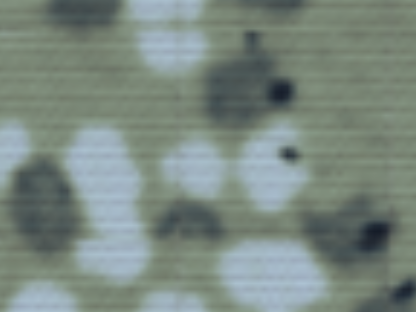
\includegraphics[width=0.3\textwidth]{imgs/checkerboard.png}
                \end{figure}
                \item Pixels at the borders of the window are not reconstructed correctly, increasing the anomaly score and the false positive rate. 
            \end{itemize}
            }
            \only<3>{
            \item Applying the autoencoder as a 256 x 256 \textbf{sliding window}:\begin{itemize}
                \item \textit{Pros}: Does not require downsampling.
                \item \textit{Cons}: Requires multiple forward passes for each image.
                \item We reduce the window stride to 128 and average the overlapping pixel predictions.
                \item We also make the implicit assumption that anomaly detection requires only local information (i.e., information within the window).
            \end{itemize}
            }
        \end{enumerate}
    \end{itemize}
\end{frame}

\begin{frame}{Losses}
    \begin{itemize}
        \item \textbf{Mean Squared Error (MSE)} 
        \begin{equation*}
            \mathcal{L}_{MSE}(x, \hat{x}) = \frac{1}{N}\sum_{i=1}^{N} (x_i - \hat{x}_i)^2
        \end{equation*} \begin{itemize}
            \item Teaches the autoencoder to reconstruct absolute pixel values.
            \item Tends to average out high-frequency details to minimize the overall loss, resulting in blurry reconstructions.
        \end{itemize}
        \item \textbf{Structural Similarity Index Measure (SSIM)} \begin{itemize}
            \item Evaluates local luminance, contrast, and structure variations within $11 \times 11$ patches.
            \begin{gather*}
                SSIM(x, \hat{x}) = \frac{(2\mu_x \mu_{\hat{x}} + c_1)(2 \sigma_{x \hat{x}} + c_2)}{(\mu_x^2 + \mu_{\hat{x}}^2 + c_1)(\sigma_x^2 + \sigma_{\hat{x}}^2 + c_2)}\\
                \mathcal{L}_{SSIM} = 1 - SSIM
            \end{gather*}
            \item Added as a complementary term to the pixel-wise $\mathcal{L}_{\text{MSE}}$ to better preserve fabric textures.
        \end{itemize}
    \end{itemize}
\end{frame}

\begin{frame}{Metrics}
    \begin{itemize}
        \item No anomalous validation set is provided for threshold calibration. Models are therefore evaluated using:
        \item \textbf{Area Under the Receiver Operating Characteristic (AUROC)} \begin{itemize}
            \item The area under the ROC curve.
            \item It represents the probability that a randomly chosen anomalous image will have a higher anomaly score than a randomly chosen normal image.
        \end{itemize}
        \item \textbf{Precision-Recall Area Under the Curve (PR AUC)}\begin{itemize}
            \item Also know as Average Precision (AP)
            \item A 1D summary of the precision-recall curve.
        \end{itemize}
    \end{itemize}
\end{frame}

\begin{frame}{CAE}
    \begin{itemize}
        \item Architecture:
            \begin{itemize}
                \item Stem: $3 \times 3$ convolution mapping the input to 16 channels.
                \item Encoder: 5 convolutional blocks; each doubles the channel depth and halves the spatial resolution.
                \item \textbf{Bottleneck:} Latent space representation of $8 \times 8 \times 512$.
                \item Decoder: 5 convolutional blocks; each halves the channel depth and doubles the spatial resolution through transposed convolutions.
                \item Head: $1 \times 1$ convolution mapping channels back to RGB.
                \item \textbf{No Skip Connections:} Omitted intentionally as they learning the identity function, and reconstruct anomalies.
            \end{itemize}
        \item Optimizer: AdamW~\cite{AdamW} with a learning rate of $10^{-3}$.
        \item Data augmentation: random horizontal and vertical flips.
        \item Trained for 50 epochs
    \end{itemize}
\end{frame}

\begin{frame}{CAE - results}
    \begin{table}
        \centering
        \footnotesize % Makes the text and tables slightly smaller
        % First Table (Left)
        \begin{minipage}{0.45\textwidth}
            \centering
            \begin{tabular}{|c|c|c|}
            \hline
                & Resize & Sliding window\\
            \hline
            MSE & 0.61 & 0.67\\
            \hline
            SSIM+MSE & 0.63 & \textbf{0.68}\\
            \hline
            \end{tabular}
            \caption{AUROC scores}
        \end{minipage}
        \hspace{0.5cm}
        % Second Table (Right)
        \begin{minipage}{0.45\textwidth}
            \centering
            \begin{tabular}{|c|c|c|}
            \hline
                & Resize & Sliding window\\
            \hline
            MSE & 0.61 & 0.69\\
            \hline
            SSIM+MSE & 0.61 & \textbf{0.71}\\
            \hline
            \end{tabular}
            \caption{PR AUC scores}
        \end{minipage}
    \end{table}
    \begin{figure}
        \centering
        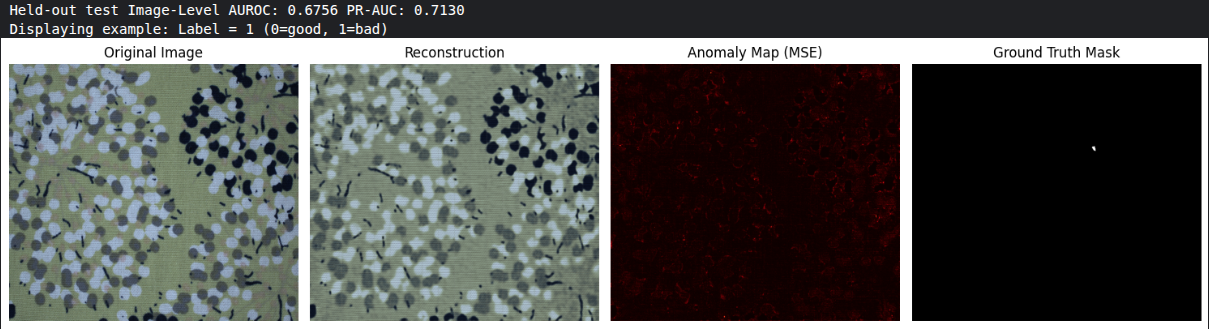
\includegraphics[width=0.8\textwidth]{imgs/cae_predictions.png}
    \end{figure}
    \begin{itemize}
        \item Performance analysis:
        \begin{itemize}
            \item Suboptimal results due to the difficulty of distinguishing between anomalies and misreconstructions.
            \item \textbf{Low-contrast anomalies} get low anomaly scores.
            \item \textbf{High variability in normal data} causes reconstruction errors in non-anomalous regions.
        \end{itemize}
    \end{itemize}

\end{frame}

\begin{frame}{CAE - ablation study}
    TODO: Inserire tabelle

    \begin{itemize}
        \item AUROC on MVTec AD~\cite{MVTecAD1} bottles is almost 0.85
    \end{itemize}
    \begin{figure}
        \centering
        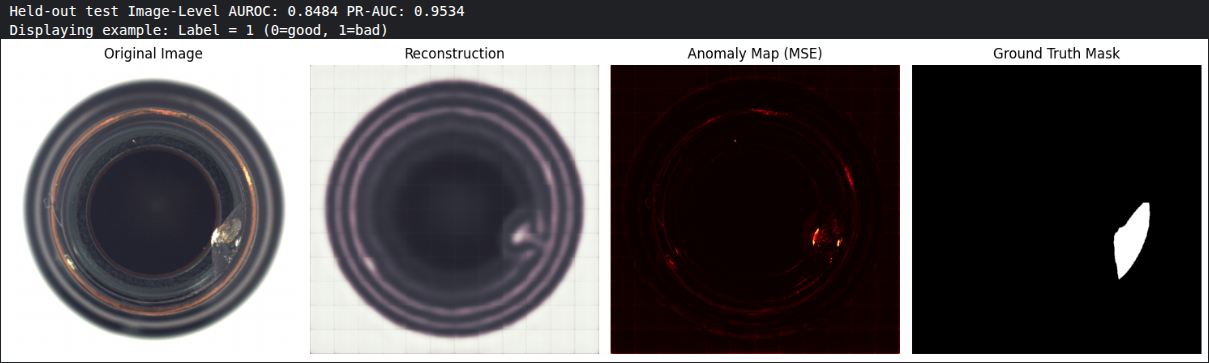
\includegraphics[width=1\textwidth]{imgs/bottle.png}
    \end{figure}
\end{frame}

\begin{frame}{VAE}
    
\end{frame}

\begin{frame}{Conclusion}
    
\end{frame}

\begin{frame}{References}
    \printbibliography
\end{frame}

\end{document}
